\documentclass[11pt]{article}
\usepackage[a4paper,margin=2.5cm]{geometry}
\usepackage[T1]{fontenc}
\usepackage[utf8]{inputenc}
\usepackage{amsmath,amssymb}
\usepackage{booktabs,array}
\usepackage{graphicx}
\usepackage{xcolor}
\usepackage{listings}
\usepackage[numbers,sort&compress]{natbib}
\usepackage[colorlinks=true,linkcolor=blue!50!black,citecolor=blue!50!black,urlcolor=blue!50!black]{hyperref}
\lstset{basicstyle=\ttfamily\small,columns=fullflexible,frame=single,framerule=0.3pt,
  rulecolor=\color{black!30},xleftmargin=4pt,xrightmargin=4pt}

\newcommand{\qZ}{qg_Z}

\title{Entrenar redes neuronales cuánticas para hardware\\ limitado por T1: qué hace y qué no hace\\ el filtro de simetría qg}
\author{Vicente Humberto Monteverde\\
\small Universidad del Museo Social Argentino (UMSA), Argentina\\
\small ORCID 0000-0001-8884-4811}
\date{\small Borrador del 2 de octubre de 2026}

\renewcommand{\figurename}{Figura}
\renewcommand{\tablename}{Tabla}
\renewcommand{\refname}{Referencias}
\renewcommand{\abstractname}{Resumen}

\begin{document}
\sloppy
\maketitle

\begin{abstract}
Una red neuronal cuántica (QNN) construida con compuertas que conservan el peso de Hamming mantiene sus datos
en un sector de peso, así que los disparos que salieron del sector pueden descartarse en la lectura. Este es el
filtro qg de la librería qang~\cite{monteverde2026qang,monteverde2026witness}. Mostramos que, con igual
amortiguamiento de amplitud (T1) en todos los qubits, la lectura filtrada de una red así es exactamente la
lectura sin ruido, en cualquier sector de peso. La fracción de disparos conservados es $(1-\gamma)^{k\,d}$ para
peso $k$ y profundidad $d$, y entrenar bajo T1 con el filtro da exactamente los parámetros del entrenamiento sin
ruido. Luego medimos cuánto vale esto en cuatro conjuntos de clasificación pequeños. Cada resultado se reporta
con el filtro y sin él, y cada predicción quedó registrada antes de su corrida, fallas incluidas. En 60 corridas
por modelo, una red entrenada en simulador y ejecutada bajo T1 gana $+2.5$ puntos con el filtro en peso~1
(IC 95\,\% $[0.8,4.1]$) y $+16.5$ puntos en peso~2 ($[11.8,21.2]$), y recupera exactamente su precisión sin
ruido. Una red entrenada con el ruido calibrado sin el filtro la alcanza (diferencias de $0.1$ puntos), y el
filtro no corrige ni el desfase ni un T1 distinto entre qubits. Estos modelos son simulables clásicamente y no
se afirma ventaja cuántica. El filtro es una manera de hacer válido el entrenamiento sin ruido bajo relajación,
con un costo en disparos conocido de antemano. Los modelos se publican como \texttt{qang.qml} (versión 0.6.0,
\texttt{pip install qang}).
\end{abstract}

\section{Introducción}

Los clasificadores cuánticos variacionales se entrenan en simuladores y se ejecutan en equipos con ruido, o se
entrenan directamente con el ruido del equipo. El entrenamiento consciente del ruido~\cite{wang2022quantumnat}
es el remedio habitual cuando ambos difieren. La verificación de simetría~\cite{bonetmonroig2018,mcardle2019}
es otro remedio: cuando el circuito ideal conserva una cantidad, se descartan los resultados que la violan. El
proyecto qang expresa las lecturas de qubits en unidades qg ($\qZ=\langle\sigma_z\rangle$ y sus
compañeras)~\cite{monteverde2026qang}. Construyó un testigo de media de registro y un filtro por disparo para
circuitos que conservan un peso de Hamming~\cite{monteverde2026witness}. Esta nota hace una pregunta acotada:
para una QNN que conserva el peso, ¿cuánto cambia ese filtro la precisión de un clasificador en hardware
limitado por T1, y cuándo deja de importar?

Respondemos con simulación exacta, un protocolo fijo y una comparación explícita. Cada lectura se toma con qang
(filtrada) y sin qang (cruda), sobre los mismos parámetros entrenados o la misma inicialización. Las
predicciones de cada estudio quedaron registradas en el repositorio antes de la corrida que las puso a prueba.
De 27 predicciones pre-registradas en los estudios que se resumen aquí, 22 se cumplieron y 5 fallaron; las
fallas se reportan junto a los aciertos.

\section{Modelo y teoría}

\paragraph{QNN que conserva el peso.} En $n$ qubits, una compuerta RBS (\emph{reconfigurable beam splitter})
actúa sobre un par $(a,b)$ como una rotación de Givens entre $|10\rangle$ y $|01\rangle$ y deja fijos
$|00\rangle$ y $|11\rangle$, así que conserva el peso de Hamming~\cite{landman2022}. Usamos $n=5$ y tres capas
de compuertas RBS sobre los pares $\{(0,1),(2,3)\}$, $\{(1,2),(3,4)\}$, $\{(4,0)\}$. Eso da 15 ángulos y
profundidad $d=9$ (subcapas). La lectura es $z=\sum_i c_i\,\qZ^{(i)}+b$ con $c_i,b$ entrenables y pérdida
logística.

\paragraph{Codificaciones.} Con cuatro variables $x\in[-1,1]^4$ sea $v=(x,1)/\|(x,1)\|$; la componente
constante conserva $\|x\|$. El modelo E (peso~1) pone $v_i$ en el estado base con el qubit $i$ excitado. El
modelo W (peso~2) pone $v_iv_j$ en el estado con los qubits $i<j$ excitados, normalizado. Los sectores tienen
dimensión 5 y 10.

\paragraph{El filtro.} Con qang, la lectura conserva solo los disparos cuyo peso es igual al peso de entrada
$k$ y renormaliza (\texttt{qang.sectors.filter\_distribution}). Sin qang, se usan todos los disparos.

\paragraph{F1/F4: exactitud con T1 igual.} Sea un amortiguamiento de amplitud con probabilidad $\gamma$ en cada
qubit después de cada subcapa. Su operador de Kraus sin salto multiplica un estado base con $k$ excitaciones por
$(1-\gamma)^{k/2}$: el mismo factor para todos los estados del sector de peso $k$. Todo salto baja el peso y sale
del sector. Las compuertas que conservan el peso nunca devuelven un estado rebajado. Por eso, condicionado a que
el peso sea $k$, el estado es exactamente el sin ruido, y
\begin{equation}
  \text{fracción conservada}=(1-\gamma)^{k\,d}.
\end{equation}
Para $\gamma=0.08$ y $d=9$ es $0.472$ en peso~1 y $0.223$ en peso~2. Si el amortiguamiento cambia entre qubits,
el factor sin salto es $\prod_{q\in S}(1-\gamma_q)^{1/2}$ sobre el conjunto excitado $S$, que no es uniforme, y se
pierde la exactitud. El desfase conserva el peso, así que el filtro no lo ve.

\paragraph{F3: entrenamiento.} Como la lectura filtrada bajo T1 es igual a la sin ruido para cualquier valor de
los parámetros, la pérdida y todos los gradientes son idénticos. Entrenar bajo T1 con el filtro da los
parámetros del entrenamiento sin ruido, con la misma inicialización.

\paragraph{F2: simulabilidad.} En peso~1 la red es una matriz ortogonal $O$ de $5\times5$ sobre $v$, y $z$ es una
forma cuadrática en $v$. En peso $k$ el sector tiene dimensión $\binom{n}{k}$, polinomial para $k$ fijo. Estos
modelos se pueden simular clásicamente. Si versiones más grandes y de mayor peso dejarían de serlo es otra
pregunta~\cite{cerezo2023simulability} que esta nota no aborda.

\section{Métodos}

Conjuntos de datos (binarios): iris (versicolor contra virginica), cáncer de mama, vino (clases 0 contra 1) y
dígitos (3 contra 8), con 100 muestras por clase cuando hay. Cada corrida usa una partición estratificada
70/30, estandarización, PCA a cuatro componentes donde hace falta y escalado a $[-1,1]$; una muestra de prueba
vale 2--3 puntos. El entrenamiento usa Adam durante 120 épocas, con gradientes por diferencias centrales en los
ángulos. Las condiciones de ruido se aplican después de cada subcapa: T1 igual con $\gamma=0.08$; T1 desigual
con $\gamma_q$ de 0.04 a 0.12 (media 0.08); y T1 igual más un cambio de fase con probabilidad 0.03. La
simulación es exacta. T1 y desfase mantienen la matriz densidad diagonal por bloques según el peso de Hamming,
así que se propaga un bloque por peso; se verificó contra la matriz densidad completa a $10^{-12}$. Protocolo:
el script de cada estudio, con sus predicciones escritas en el encabezado, se registró antes de usar la semilla
de su corrida reportada; el código se depuró con otra semilla y pocas épocas. Los hashes de los commits están en
las notas de investigación~\cite{monteverde2026qang}.

\section{Resultados}

\paragraph{Estudios con una semilla.} La QNN que conserva el peso y la norma llega a una precisión media de
0.960 sobre los cuatro conjuntos. Queda a la par de una QNN estándar de cuatro qubits que no conserva el peso
(0.952), de una máquina de vectores soporte RBF (0.957) y de una red MLP pequeña (0.961). Sin la componente de
norma, la misma red obtiene 0.791. Entrenada sin ruido y ejecutada bajo T1 con el filtro, conserva exactamente su
precisión sin ruido. Entrenar bajo T1 con el filtro reproduce el entrenamiento sin ruido a $5\times10^{-9}$ en los
parámetros (F3). Con $\gamma=0.08$, una QNN estándar entrenada sin ruido colapsa bajo T1 (0.771); entrenada bajo
T1 se recupera (0.944).

Las predicciones que fallaron:
\begin{itemize}
\item la codificación arccos no mejoró la precisión;
\item el gemelo cuadrático clásico no quedó a menos de 1 punto de la QNN con la regularización por defecto;
\item el T1 desigual le costó al filtro 1.5 puntos en una corrida (límite: 1 punto);
\item el peso~2 fue menos preciso que el peso~1 (por 3.7 puntos);
\item entrenado bajo T1, el modelo de peso~2 sin filtro quedó 0.6 puntos por delante del filtrado.
\end{itemize}

\paragraph{Réplica en 60 corridas.} Las comparaciones clave se repitieron con 5 semillas $\times$ 3 particiones
$\times$ 4 conjuntos. La Tabla~\ref{tab:main} y la Fig.~\ref{fig:main} dan los resultados; las cinco
predicciones pre-registradas de esta réplica se cumplieron.

\begin{table}[h]
\centering\small
\begin{tabular}{lcccc}
\toprule
 & \multicolumn{2}{c}{E (peso 1)} & \multicolumn{2}{c}{W (peso 2)}\\
lectura & con qang & sin qang & con qang & sin qang\\
\midrule
exacta (sin ruido) & 0.952 & & 0.922 & \\
T1, entrenada sin ruido & 0.952 & 0.928 & 0.922 & 0.757\\
T1, entrenada con el ruido & 0.952 & 0.951 & 0.922 & 0.924\\
T1 desigual, entrenada sin ruido & 0.947 & 0.921 & 0.916 & 0.732\\
desfase, entrenada sin ruido & 0.918 & 0.792 & 0.882 & 0.656\\
desfase, entrenada con el ruido & 0.950 & & 0.926 & \\
\bottomrule
\end{tabular}
\caption{Precisión de prueba media en 60 corridas por modelo, con y sin el filtro qg.}
\label{tab:main}
\end{table}

\begin{figure}[h]
\centering
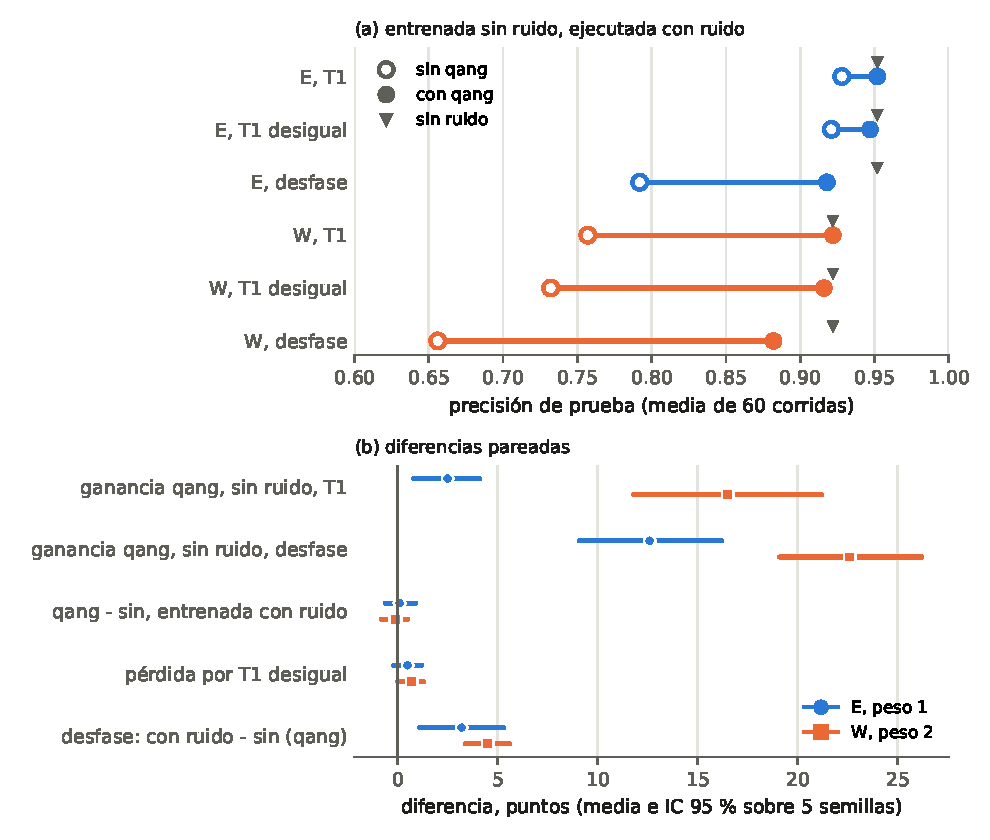
\includegraphics[width=0.86\textwidth]{../qml/fig_qml_es.pdf}
\caption{(a) Precisión de redes entrenadas sin ruido y ejecutadas con ruido, sin (vacío) y con (lleno) el
filtro; los triángulos marcan la precisión sin ruido. (b) Diferencias pareadas, media e IC 95\,\% sobre
5 semillas.}
\label{fig:main}
\end{figure}

Las diferencias pareadas (media, IC 95\,\% entre semillas) fueron las siguientes.
\begin{itemize}
\item \textit{Ganancia del filtro, entrenada sin ruido, bajo T1:} $+2.5$ $[0.8,4.1]$ puntos (E) y
  $+16.5$ $[11.8,21.2]$ (W). El modelo filtrado quedó adelante o empatado en 50/60 (E) y 56/60 (W) corridas.
\item \textit{Con entrenamiento con ruido:} $+0.1$ $[-0.6,0.9]$ (E) y $-0.1$ $[-0.8,0.5]$ (W).
\item \textit{Pérdida por T1 desigual:} $0.5$ $[-0.2,1.2]$ (E) y $0.7$ $[0.0,1.3]$ (W). Los 1.5 puntos de la
  corrida anterior estaban en el extremo alto de la dispersión.
\item \textit{Desfase, entrenamiento con ruido menos sin ruido, con filtro:} $+3.2$ (E) y $+4.5$ (W), ambos
  IC por encima de 0.
\item \textit{Con desfase, un modelo entrenado sin ruido igual gana} $+12.6$ (E) y $+22.6$ (W) puntos con el
  filtro, que elimina la parte T1 del ruido combinado.
\item \textit{Peso~2 frente a peso~1:} $-3.0$ $[-4.0,-2.0]$ puntos.
\end{itemize}

\section{Discusión}

La diferencia que hace el filtro depende de cómo se entrenó la red. Entrenada en simulador y ejecutada con
relajación, el filtro es decisivo. Su efecto crece con el peso, porque un estado de peso $k$ decae $k$ veces más
rápido. Entrenada con un modelo de ruido calibrado, una red sin filtro aprende el decaimiento, y el filtro no
agrega nada medible. Lo que aporta el filtro es, por lo tanto, de procedimiento y no una ganancia de precisión
sobre la mejor alternativa. Con T1 igual hace exactamente válido el entrenamiento sin ruido, sin modelo de ruido
ni corridas de entrenamiento con ruido, y su costo (los disparos descartados) se conoce antes de ejecutar. El T1
desigual y el desfase no se corrigen. En hardware con mucha dispersión de T1 o desfase fuerte, el filtro
complementa un modelo de ruido y no lo reemplaza.

\paragraph{Limitaciones.} Todo el ruido es simulado. Hay una arquitectura por peso, cinco qubits y conjuntos
pequeños en los que una muestra de prueba vale 2--3 puntos. La codificación de peso~2 es una elección entre
muchas, y no aprovechó bien el sector más grande. No se afirma ventaja cuántica: estas redes son simulables
clásicamente. Una corrida en hardware con el filtro es la siguiente prueba natural.

\section*{Disponibilidad de código y datos}

Modelos: \texttt{qang.qml} en \texttt{qang} 0.6.0 (\texttt{pip install qang}), solo NumPy, con
\texttt{WeightQNN}, \texttt{kept\_fraction} y \texttt{compare\_qang}. Estudios: \texttt{examples/qnn\_*\_qg.py} y
RESEARCH\_NOTES \S75--\S80, con pruebas en \texttt{tests/}. Los cuadernos Colab
\texttt{notebooks/qang\_qml\_es.ipynb} (español) y \texttt{qang\_qml.ipynb} (inglés) instalan la librería desde
PyPI. Repositorio: \url{https://github.com/Viny2030/qang}.

\begin{lstlisting}[language=Python]
from qang.qml import WeightQNN
m = WeightQNN(n_qubits=5, weight=2).fit(X_train, y_train)
m.score(X_test, y_test, gamma=0.08, qang=True)   # = precision sin ruido
m.score(X_test, y_test, gamma=0.08, qang=False)  # lectura cruda
\end{lstlisting}

\bibliographystyle{unsrtnat}
\bibliography{../refs}

\end{document}
